\documentclass[12pt]{article}
\usepackage[letterpaper, margin=1in]{geometry}
\usepackage{graphicx}
\usepackage{subcaption}
\graphicspath{{./Figures/}}
\usepackage{hyperref}
\usepackage{parskip}
\usepackage{amsmath}
\usepackage{amssymb}
\usepackage{mathrsfs}
\usepackage{enumitem}
\allowdisplaybreaks

\title{ELECENG 3CL4 Lab 3 Pre-lab}
\author{
    Aaron Pinto \\
    pintoa9 \\
    L02
    \and
    Raeed Hassan \\
    hassam41 \\
    L02
}

\begin{document}

\maketitle
\clearpage

\section{Proportional Control of DC Motor}
\textbf{Pre-Lab Question 1} \\
The closed-loop transfer function $T(s)$ is:
\begin{equation*}
\begin{aligned}[b]
    T(s) &= \frac{G(s)G_c(s)}{1 + G(s)G_c(s)} \\
    &= \frac{k_pG(s)}{1 + k_pG(s)}
\end{aligned}
\end{equation*}
We find the characteristic equation of the closed-loop transfer function $T(s)$ by equating the denominator of the transfer function to zero below: 
\begin{equation*}
\begin{aligned}[b]
    0 &= 1 + k_pG(s) \\
    0 &= 1 + \frac{k_pA}{s(s\tau_m + 1)} \\
    0 &= 1 + \frac{k_pA}{s^2\tau_m + s} \\
    -1 &= \frac{k_pA}{s^2\tau_m + s} \\
    -s^2\tau_m - s &= k_pA \\
    0 &= s^2\tau_m + s + k_pA
\end{aligned}
\end{equation*}
The closed-loop poles of the system are found by determining the poles of the characteristic equation, which is done in Equation~\ref{eq:q1}. The poles have a constant real term, and a term that is real for $k_p < \frac{1}{4A\tau_m}$ and imaginary for $k_p > \frac{1}{4A\tau_m}$. 
\begin{equation} \label{eq:q1}
\begin{aligned}[b]
    p_{1,2} &= \frac{-b \pm \sqrt{b^2 - 4ac}}{2a} \\
    a &= \tau_m, \ b = 1, \ c = k_pA \\
    &= \frac{-1 \pm \sqrt{1 - 4\tau_m k_p A}}{2\tau_m} \\
    p_{1,2} &= -\frac{1}{2\tau_m} \pm \frac{1}{2\tau_m}\sqrt{1 - 4k_p A \tau_m}
\end{aligned}
\end{equation}

\textbf{Pre-Lab Question 2} \\
The path of the poles $p_{1,2}$ in the s-plane as $k_p$ approaches infinity are shown in Figure~\ref{fig:q2}. The two poles start wholly real, approaching $-\frac{1}{2\tau_m}$ as $k_p$ approaches $\frac{1}{4A\tau_m}$. When the value of $k_p$ is greater than $\frac{1}{4A\tau_m}$, the poles have a constant real part $-\frac{1}{2\tau_m}$ and an increasing/decreasing imaginary part which creates vertical paths for the poles in the s-plane.
\begin{figure}[h!]
    \centering
    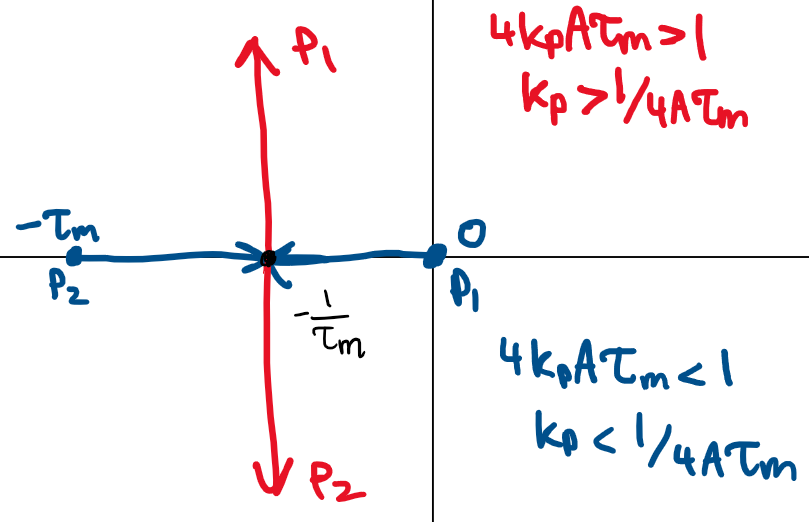
\includegraphics[width=0.8\textwidth]{q2}
    \caption{\label{fig:q2}The path of the closed-loop poles as $k_p$ approaches infinity}
\end{figure} \newpage

\textbf{Pre-Lab Question 3} \\
We can rewrite the closed-loop transfer function $T(s)$ to be in the standard form of a second order system:
\begin{equation*}
\begin{aligned}[b]
    T(s) &= \frac{k_pG(s)}{1 + k_pG(s)} \\
    &= \frac{\frac{k_pA}{s^2\tau_m + s}}{1 + \frac{k_pA}{s^2\tau_m + s}} \\
    &= \frac{k_pA}{s^2\tau_m + s + k_pA} \\
    &= \frac{\frac{k_pA}{\tau_m}}{s^2 + \frac{s}{\tau_m} + \frac{k_pA}{\tau_m}}
\end{aligned}
\end{equation*}
For a second order system in the standard form:
\begin{equation*}
    F_2(s) = \frac{\omega_n^2}{s^2 + 2\zeta\omega_ns + \omega_n^2}
\end{equation*}
We can determine the parameters $\zeta\omega_n$, $\omega_n$, and $\zeta$ in Equation~\ref{eq:q3} from $T(s)$.
\begin{align*}
    \omega_n^2 &= \frac{k_pA}{\tau_m} & 2\zeta\omega_ns &= \frac{s}{\tau_m} & \zeta &= \frac{1}{2\tau_m\omega_n} \\
    \omega_n &= \sqrt{\frac{k_pA}{\tau_m}} & \zeta\omega_n &= \frac{1}{2\tau_m} & \zeta &= \frac{1}{2\sqrt{k_pA\tau_m}} \stepcounter{equation}\tag{\theequation}\label{eq:q3}
\end{align*}

\textbf{Pre-Lab Question 4} \\
When the controller gain $k_p = \frac{1}{4A\tau_m}$, we can show the system is critically damped by determining $\zeta = 1$ in Equation~\ref{eq:q4}.
\begin{equation} \label{eq:q4}
\begin{aligned}[b]
    \zeta &= \frac{1}{2\sqrt{k_pA\tau_m}} \\
    &= \frac{1}{2\sqrt{\frac{A\tau_m}{4A\tau_m}}} \\
    &= \frac{1}{2\sqrt{\frac{1}{4}}} \\
    &= \frac{1}{2(0.5)} \\
    \zeta &= 1
\end{aligned}
\end{equation}

\textbf{Pre-Lab Question 5} \\
We can use the expression for the closed-loop poles found previously to write the pole positions as Equation~\ref{eq:q5} for $k_p > \frac{1}{4A\tau_m}$. 
\begin{equation} \label{eq:q5}
\begin{aligned}[b]
    p_{1,2} &= -\frac{1}{2\tau_m} \pm \frac{1}{2\tau_m}\sqrt{1 - 4k_p A \tau_m} \\
    &= \frac{1}{2\tau_m} \left( -1 \pm \sqrt{1 - 4k_p A \tau_m} \right) \\
    &= \frac{1}{2\tau_m} \left( -1 \pm j\sqrt{4k_p A \tau_m - 1} \right) \\
    &= \frac{1}{2\tau_m} \left( -1 \pm j\sqrt{\frac{1 - \frac{1}{4k_pA\tau_m}}{\frac{1}{4k_pA\tau_m}}} \right) \\
    &= \frac{1}{2\tau_m} \left( -1 \pm j\sqrt{\frac{1 - \left(\frac{1}{2\sqrt{k_pA\tau_m}}\right)^2}{\left(\frac{1}{2\sqrt{k_pA\tau_m}}\right)^2}} \right) \\
    &= \frac{1}{2\tau_m} \left( -1 \pm j\sqrt{\frac{1 - \zeta^2}{\zeta^2}} \right) \\
    &= \frac{1}{2\tau_m} \left( -1 \pm j{\frac{\sqrt{1 - \zeta^2}}{\zeta}} \right) \\
    &= \frac{1}{2\tau_m} \left( -1 \pm j\tan(\cos^{-1}(\zeta))\right) \\ % by the power of the trig gods
\end{aligned}
\end{equation}

\section{Trade-offs in Proportional Control of a Servomotor: Theoretical Insight}
\textbf{Pre-Lab Question 6} \\
Using the provided expressions and values for $\omega_n$ and $zeta$, we can show that the closed-loop system in the Figure will have the following $T_s$, $P.O.$ and $T_{r1}$ when underdamped:
\begin{align*}
    T_s &\approx \frac{4}{\zeta\omega_n} \\
    &\approx \frac{4}{\frac{\omega_n}{2\omega_n\tau_m}} \\
    &\approx \frac{4}{\frac{1}{2\tau_m}} \\
    &\approx 8\tau_m \\
    P.O. &= 100\exp\left(-\frac{\pi\zeta}{\sqrt{1-\zeta^2}}\right) \\
    &= 100\exp\left(-\frac{\frac{\pi}{2\omega_n\tau_m}}{\sqrt{1-\left(\frac{1}{2\omega_n\tau_m}\right)^2}}\right) \\
    &= 100\exp\left(-\frac{\frac{\pi}{2\omega_n\tau_m}}{\sqrt{1-\frac{1}{4\omega_n^2\tau_m^2}}}\right) \\
    &= 100\exp\left(-\frac{\pi}{2\omega_n\tau_m\sqrt{1-\frac{1}{4\omega_n^2\tau_m^2}}}\right) \\
    % &= 100\exp\left(-\frac{\pi}{2\omega_n\tau_m\sqrt{\frac{4\omega_n^2\tau_m^2}{4\omega_n^2\tau_m^2}-\frac{1}{4\omega_n^2\tau_m^2}}}\right) \\
    &= 100\exp\left(-\frac{\pi}{2\omega_n\tau_m\sqrt{\frac{4\omega_n^2\tau_m^2 - 1}{4\omega_n^2\tau_m^2}}}\right) \\
    &= 100\exp\left(-\frac{\pi}{2\omega_n\tau_m\frac{\sqrt{4\omega_n^2\tau_m^2 - 1}}{\sqrt{4\omega_n^2\tau_m^2}}}\right) \\
    &= 100\exp\left(-\frac{\pi}{\sqrt{4\omega_n^2\tau_m^2 - 1}}\right) \\
    &= 100\exp\left(-\frac{\pi}{\sqrt{4\frac{k_pA}{\tau_m}\tau_m^2 - 1}}\right) \\
    &= 100\exp\left(-\frac{\pi}{\sqrt{4k_pA\tau_m - 1}}\right) \\
    T_{r1} &\approx \frac{2.16\zeta + 0.6}{\omega_n} \\
    &\approx \frac{\frac{2.16}{2\omega_n\tau_m} + 0.6}{\omega_n} \\
    &\approx \frac{\frac{2.16 + 1.2\omega_n\tau_m}{2\omega_n\tau_m}}{\omega_n} \\
    &\approx \frac{2.16 + 1.2\omega_n\tau_m}{2\omega_n^2\tau_m} \\
    &\approx \frac{2.16 + 1.2\sqrt{\frac{k_pA}{\tau_m}}\tau_m}{2\frac{k_pA}{\tau_m}\tau_m} \\
    &\approx \frac{2.16 + 1.2\sqrt{k_pA\tau_m}}{2k_pA} \\
\end{align*}

\textbf{Pre-Lab Question 7} \\
$T_s$ does not change with $k_p$. P.O. increases as $k_p$ increases and it approaches a horizontal asymptote of 100\%, which is the expected behaviour for an underdamped system. $T_{r1}$ decreases as $k_p$ decreases and approaches the horizontal asymptote of 0.

\textbf{Pre-Lab Question 8} \\
The 2\% settling time $T_s$ cannot be controlled through $k_p$, while the percent overshoot and the 10\% to 90\% rise time $T_{r1}$ can.

\textbf{Pre-Lab Question 9} \\
From the block diagram from Figure 1 in the lab document, you can determine the total output response to the reference and disturbance inputs as Equation~\ref{eq:q9}.
\begin{equation} \label{eq:q9}
\begin{aligned}[b]
    \Theta(s) &= \frac{k_pG(s)}{1 + k_pG(s)}R(s) + \frac{G(s)}{1 + k_pG(s)}T_d(s) \\
    &= \frac{\frac{k_pA}{s(s\tau_m + 1)}}{1 + \frac{k_pA}{s(s\tau_m + 1)}}R(s) + \frac{\frac{A}{s(s\tau_m + 1)}}{1 + \frac{k_pA}{s(s\tau_m + 1)}}T_d(s) \\
    &= \frac{\frac{k_pA}{s(s\tau_m + 1)}}{\frac{s(s\tau_m + 1) + k_pA}{s(s\tau_m + 1)}}R(s) + \frac{\frac{A}{s(s\tau_m + 1)}}{\frac{s(s\tau_m + 1) + k_pA}{s(s\tau_m + 1)}}T_d(s) \\
    &= \frac{k_pA}{s(s\tau_m + 1) + k_pA}R(s) + \frac{A}{s(s\tau_m + 1) + k_pA}T_d(s) \\
    &= \frac{k_pA}{s^2\tau_m + s + k_pA}R(s) + \frac{A}{s^2\tau_m + s + k_pA}T_d(s) \\
    &= \frac{\frac{k_pA}{\tau_m}}{s^2 + \frac{1}{\tau_m}s + \frac{k_pA}{\tau_m}}R(s) + \frac{\frac{A}{\tau_m}}{s^2 + \frac{1}{\tau_m}s + \frac{k_pA}{\tau_m}}T_d(s)
\end{aligned}
\end{equation} \newpage

\textbf{Pre-Lab Question 10} \\
To find the steady-state error to a step input $R(s) = \frac{\theta_d}{s}$ in absence of disturbance, calculate the steady-state error of the reference input term using the final limit theorem in Equation~\ref{eq:q10}.
\begin{equation} \label{eq:q10}
\begin{aligned}[b]
    e_{ss} &= \lim_{s \to 0} \ s \frac{1}{1 + G_c(s)G(s)} R(s) \\
    &= \lim_{s \to 0} \ s \frac{1}{1 + G_c(s)G(s)} \frac{\theta_d}{s} \\
    &= \lim_{s \to 0} \ \frac{\theta_d}{1 + G_c(s)G(s)} \\
    &= \frac{\theta_d}{1 + \text{lim}_{s \to 0} \ G_c(s)G(s)} \\
    &= \frac{\theta_d}{1 + \text{lim}_{s \to 0} \ \frac{k_pA}{s(s\tau_m + 1)}} \\
    &= \frac{\theta_d}{1 + (\text{lim}_{s \to 0} \ \frac{k_pA}{s(s\tau_m + 1)}\to \infty)} \\
    e_{ss} &= 0
\end{aligned}
\end{equation}
The feedback gain $k_p$ does not have any effect on this error, because the system is type 1.

\textbf{Pre-Lab Question 11} \\
To find the steady-state error to a step input $R(s) = \frac{\theta_d}{s}$ in the presence of a constant disturbance $T_d(s) = \frac{\tau_d}{s}$, calculate the steady-state error of the reference input term using the final limit theorem in Equation~\ref{eq:q11}.
\begin{align*}
    E(s) &= R(s) - Y(s) \\
    &= R(s) - \left(\frac{k_pG(s)}{1 + k_pG(s)}R(s) + \frac{G(s)}{1 + k_pG(s)}T_d(s) \right) \\
    &= R(s) - \frac{k_pG(s)R(s) - G(s)T_d(s)}{1 + k_pG(s)} \\
    &= \frac{R(s) + k_pG(s)R(s)}{1 + k_pG(s)} - \frac{k_pG(s)R(s) - G(s)T_d(s)}{1 + k_pG(s)} \\
    % &= \frac{R(s) + k_pG(s)R(s) - k_pG(s)R(s) - G(s)T_d(s)}{1 + k_pG(s)} \\
    &= \frac{R(s) - G(s)T_d(s)}{1 + k_pG(s)} \\
    e_{ss} &= \lim_{s \to 0} \ s \frac{1}{1 + k_pG(s)} \frac{\theta_d}{s} - \lim_{s \to 0} \ s \frac{G(s)}{1 + k_pG(s)} \frac{\tau_d}{s} \\
    &= 0 - \lim_{s \to 0} \ \frac{G(s)}{1 + k_pG(s)} \tau_d \\
    &= - \lim_{s \to 0} \ \frac{G(s)}{1 + k_pG(s)} \tau_d \\
    &= - \lim_{s \to 0} \ \frac{\frac{A}{s(s\tau_m + 1)}}{1 + \frac{k_pA}{s(s\tau_m + 1)}} \tau_d \\
    &= - \lim_{s \to 0} \ \frac{A}{s(s\tau_m + 1) + k_pA} \tau_d \\
    &= - \frac{A\tau_d}{k_pA + \lim_{s \to 0} \ s(s\tau_m + 1)} \\
    &= - \frac{A\tau_d}{k_pA + (\lim_{s \to 0} \ s(s\tau_m + 1) \to 0)} \\
    &= - \frac{A\tau_d}{k_pA} \\
    &= - \frac{\tau_d}{k_p} \stepcounter{equation}\tag{\theequation}\label{eq:q11}
\end{align*}
A larger feedback gain $k_p$ makes the error smaller, and vice versa, because $k_p$ is inversely proportional to this error.

\setcounter{section}{5}
\section{Proportional Controller with Velocity Feedback}
\textbf{Pre-Lab Question 12} \\
The block diagram of the proportional control of the servomotor with additional velocity feedback can be transformed using block diagram transforms as shown in Figure~\ref{fig:q12}. From the block diagram, we can see that the total output response when $F(s) \approx 1$ can be written as Equation~\ref{eq:q12}.
\begin{equation} \label{eq:q12}
\begin{aligned}[b]
    \Theta(s) &= \frac{k_pG(s)}{1 + k_vsG(s) + k_pG(s)}R(s) + \frac{G(s)}{1 + k_vsG(s) + k_pG(s)}T_d(s) \\
    &= \frac{\frac{k_pA}{s(s\tau_m + 1)}}{1 + s\frac{k_vA}{s(s\tau_m + 1)} + \frac{k_pA}{s(s\tau_m + 1)}}R(s) + \frac{\frac{A}{s(s\tau_m + 1)}}{1 + s\frac{k_vA}{s(s\tau_m + 1)} + \frac{k_pA}{s(s\tau_m + 1)}}T_d(s) \\
    &= \frac{k_pA}{s(s\tau_m + 1) + k_vAs + kpA}R(s) + \frac{A}{s(s\tau_m + 1) + k_vAs + kpA}T_d(s) \\
    &= \frac{\frac{k_pA}{\tau_m}}{s^2 + \frac{1+k_vA}{\tau_m}s + \frac{k_pA}{\tau_m}}R(s) + \frac{\frac{A}{\tau_m}}{s^2 + \frac{1+k_vA}{\tau_m}s + \frac{k_pA}{\tau_m}}T_d(s)
\end{aligned}
\end{equation}
\begin{figure}[h!]
    \centering
    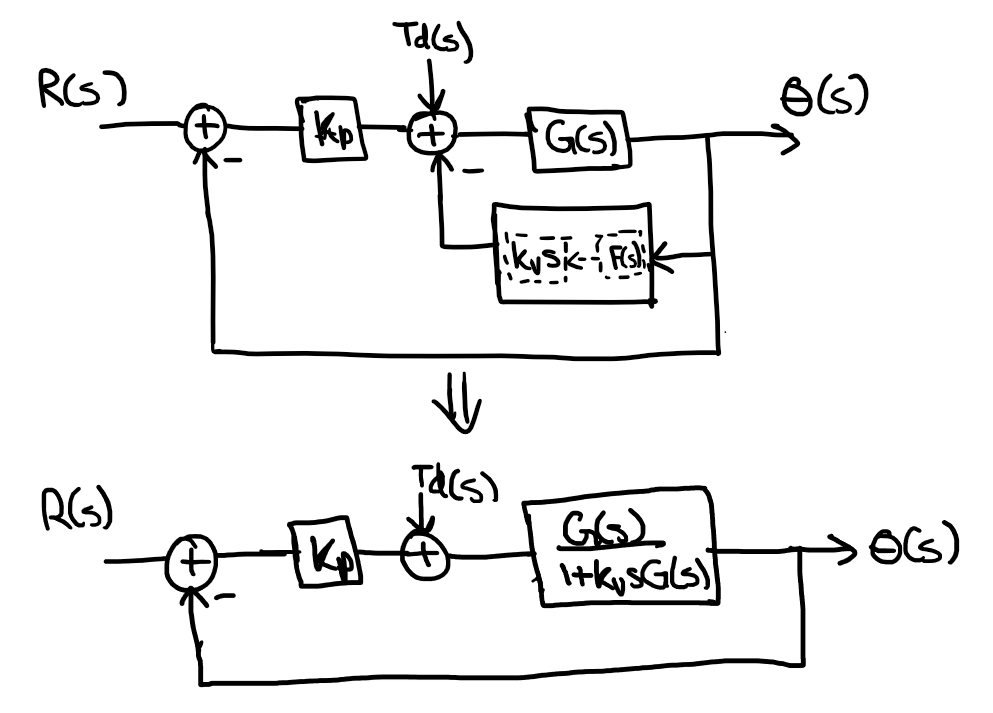
\includegraphics[width=\textwidth]{q12}
    \caption{\label{fig:q12}The block diagram transformation of the servomotor with additional velocity feedback}
\end{figure}

\textbf{Pre-Lab Question 13} \\
The steady-state error due to a step disturbance can be calculated through the final limit theorem as shown in Equation~\ref{eq:q13}.
\begin{equation} \label{eq:q13}
\begin{aligned}[b]
    \left|e_{ss}\right| &= \lim_{s \to 0} \ s\frac{A}{s(s\tau_m+1) + k_vAs + k_pA}T_d(s) \\
    &= \lim_{s \to 0} \ s\frac{A}{s(s\tau_m+1) + k_vAs + k_pA}\frac{\tau_d}{s} \\
    &= \lim_{s \to 0} \ \frac{A\tau_d}{s(s\tau_m+1) + k_vAs + k_pA} \\
    &= \frac{A\tau_d}{k_pA + \text{lim}_{s \to 0} \ s(s\tau_m+1) + k_vAs} \\
    &= \frac{A\tau_d}{k_pA + (\text{lim}_{s \to 0} \ s(s\tau_m+1) + k_vAs \to 0)} \\
    &= \frac{A\tau_d}{k_pA} \\
    \left|e_{ss}\right|&= \frac{\tau_d}{k_p}
\end{aligned}
\end{equation} 

\textbf{Pre-Lab Question 14} \\
The closed-loop transfer function can be written as:
\begin{equation*}
\begin{aligned}[b]
    T(s) &= \frac{k_pG(s)}{1 + k_vsG(s) + k_pG(s)} \\
    &= \frac{\frac{k_pA}{s(s\tau_m + 1)}}{1 + \frac{k_vA}{s(s\tau_m + 1)}s + \frac{k_pA}{s(s\tau_m + 1)}} \\
    &= \frac{k_pA}{s^2\tau_m + (1 + k_vA)s + k_pA} \\
    &= \frac{\frac{k_pA}{\tau_m}}{s^2 + \frac{1 + k_vA}{\tau_m}s + \frac{k_pA}{\tau_m}} 
\end{aligned}
\end{equation*}
We can find $\zeta$ by writing the closed-loop transfer function in the form of a standard second order system and finding the parameters of the system in Equation~\ref{eq:q14}.
\begin{equation*}
    F_2(s) = \frac{\omega_n^2}{s^2 + 2\zeta\omega_ns + \omega_n^2}
\end{equation*}
\begin{align*}
    \omega_n^2 &= \frac{k_pA}{\tau_m} & 2\zeta\omega_ns &= \frac{1+k_vA}{\tau_m}s & \zeta &= \frac{1+k_vvA}{2\tau_m\omega_n} \\
    \omega_n &= \sqrt{\frac{k_pA}{\tau_m}} & \zeta\omega_n &= \frac{1+k_vA}{2\tau_m} & \zeta &= \frac{1+k_vA}{2\sqrt{k_pA\tau_m}} \stepcounter{equation}\tag{\theequation}\label{eq:q14}
\end{align*}

\textbf{Pre-Lab Question 15} \\
Increasing $k_p$ will decrease $\zeta$, which will lead to a decrease in the rise time and an increase in the maximum overshoot, while decreasing $k_p$ will increase the rise time and decrease the maximum overshoot. Increasing $k_v$ will increase $\zeta$, which will lead to an increase in the rise time and a decrease in the maximum overshoot, while decreasing $k_v$ will decrease the rise time and increase the maximum overshoot. The settling time is inversely proportional to $\zeta\omega_n$, which increases as $k_v$ increases and decreases as $k_v$ decreases. Therefore, the settling time increases as $k_v$ decreases and decreases as $k_v$ increases. The steady-state error to a constant disturbance is inversely proportional to $k_p$. % talk about settling time

\end{document}
